%% =========================================================================
%% Section 4: Descriptive Results and Demographic Landscape
%% =========================================================================

\section{Descriptive Results and the Demographic Landscape}

\subsection{Sociodemographic Profile of Older Indian Adults}
Table~\ref{tab:sample_char} presents the survey-weighted demographic and socioeconomic distribution of the target population ($N = 66,606$), alongside raw unweighted respondent counts.

\begin{table}[!htbp]
\centering
\begin{singlespace}
\small
\caption{\textbf{Baseline Sociodemographic and Early-Life Characteristics of Older Adults in India ($\mathbf{N=66,606}$).}}
\label{tab:sample_char}
\renewcommand{\arraystretch}{0.92}
\resizebox{\textwidth}{!}{%
\begin{tabular}{llrr c llrr}
\toprule
\multicolumn{4}{c}{\textbf{Panel A: Sociodemographic Profile}} & & \multicolumn{4}{c}{\textbf{Panel B: Economic \& Early-Life Profile}} \\
\cmidrule(lr){1-4} \cmidrule(lr){6-9}
\textbf{Domain} & \textbf{Category / Subgroup} & \textbf{Unw. N} & \textbf{Wtd. \%} & & \textbf{Domain} & \textbf{Category / Subgroup} & \textbf{Unw. N} & \textbf{Wtd. \%} \\
\midrule
Age Cohort & 45--59 years (Mid-life) & 34,704 & 49.77\% & & Household MPCE & Quintile 1 (Poorest) & 13,181 & 20.86\% \\
Age Cohort & 60--74 years (Young-old) & 25,022 & 38.80\% & & Household MPCE & Quintile 2 & 13,403 & 21.24\% \\
Age Cohort & 75+ years (Oldest-old) & 6,880 & 11.42\% & & Household MPCE & Quintile 3 & 13,371 & 20.49\% \\
\cmidrule(lr){1-4}
Sex & Female & 35,567 & 54.06\% & & Household MPCE & Quintile 4 & 13,412 & 19.42\% \\
Sex & Male & 31,039 & 45.94\% & & Household MPCE & Quintile 5 (Richest) & 13,239 & 17.99\% \\
\cmidrule(lr){1-4} \cmidrule(lr){6-9}
Residence & Rural village & 43,240 & 68.53\% & & Childhood SES & Pretty well-off financially & 4,848 & 7.77\% \\
Residence & Urban town/city & 23,366 & 31.47\% & & Childhood SES & About average & 35,438 & 49.32\% \\
\cmidrule(lr){1-4}
Social Group & General / Forward / None & 16,295 & 24.84\% & & Childhood SES & Poor & 25,605 & 42.16\% \\
Social Group & Other Backward Classes & 25,212 & 46.66\% & & Childhood SES & It varied & 394 & 0.76\% \\
\cmidrule(lr){6-9}
Social Group & Scheduled Caste (SC) & 11,014 & 19.66\% & & Childhood Health & Good / Very good & 58,272 & 87.46\% \\
Social Group & Scheduled Tribe (ST) & 11,746 & 8.84\% & & Childhood Health & Fair / Poor / Very poor & 7,369 & 12.54\% \\
\cmidrule(lr){1-4} \cmidrule(lr){6-9}
Marital Status & Married / Cohabiting & 49,949 & 73.86\% & & Bedridden ($\ge 1$ mo.) & No & 62,881 & 94.25\% \\
Marital Status & Widowed & 14,780 & 23.72\% & & Bedridden ($\ge 1$ mo.) & Yes & 3,370 & 5.75\% \\
\cmidrule(lr){6-9}
Marital Status & Divorced / Separated & 1,006 & 1.23\% & & Adversity Index & 0 adversities & 34,506 & 48.19\% \\
Marital Status & Never Married & 868 & 1.19\% & & Adversity Index & 1 adversity & 26,556 & 44.06\% \\
\cmidrule(lr){1-4}
Education & No formal education & 31,350 & 50.62\% & & Adversity Index & 2 adversities & 4,003 & 6.86\% \\
Education & Less than primary & 7,598 & 10.92\% & & Adversity Index & 3 adversities & 466 & 0.88\% \\
Education & Primary completed & 8,761 & 12.05\% & & & & & \\
Education & Middle school completed & 6,337 & 8.35\% & & & & & \\
Education & Secondary completed & 5,953 & 7.93\% & & & & & \\
Education & Higher secondary / Diploma & 3,175 & 4.94\% & & & & & \\
Education & Graduate and above & 3,429 & 5.19\% & & & & & \\
\bottomrule
\end{tabular}%
}
\end{singlespace}
\end{table}

The demographic and socioeconomic distribution depicts a population shaped by the structural realities of mid-to-late 20th-century India:
\begin{itemize}
    \item \textbf{High Illiteracy and Limited Schooling:} Over half (50.62\%) of older Indian adults have never received any formal schooling, and an additional 10.92\% completed less than primary schooling. Only 5.19\% attained a college degree or higher qualification.
    \item \textbf{Rural Predominance:} More than two-thirds (68.53\%) of the population reside in rural villages, with 31.47\% living in urban towns or cities.
    \item \textbf{Caste Composition:} Other Backward Classes (OBC) constitute the largest social group at 46.66\%, followed by General/Forward castes (24.84\%), Scheduled Castes (19.66\%), and Scheduled Tribes (8.84\%).
    \item \textbf{Gender and Marital Precarity:} Women comprise 54.06\% of the older population. Due to gender differences in life expectancy and marital age gaps, nearly a quarter (23.72\%) of all older adults are widowed, with widowhood overwhelmingly concentrated among women.
    \item \textbf{Pervasive Early-Life Deprivation:} Growing up in economic precarity was the norm rather than the exception: 42.16\% of respondents reported that their childhood family was financially poor, and 49.32\% described their background as average. Only 7.77\% grew up in relatively well-off households. Furthermore, 12.54\% reported poor general health in childhood, and 5.75\% experienced a severe illness that kept them bedridden for a month or longer before age 16.
\end{itemize}

\subsection{Outcome Prevalence across Stages of Ageing}
Table~\ref{tab:outcomes_age} and Figure~\ref{fig:outcomes_age} document the survey-weighted prevalence of depressive symptoms and cognitive impairment across three distinct stages of later life: mid-life (45--59 years), young-old (60--74 years), and the oldest-old (75 years and older). 

\begin{figure}[!htbp]
    \centering
    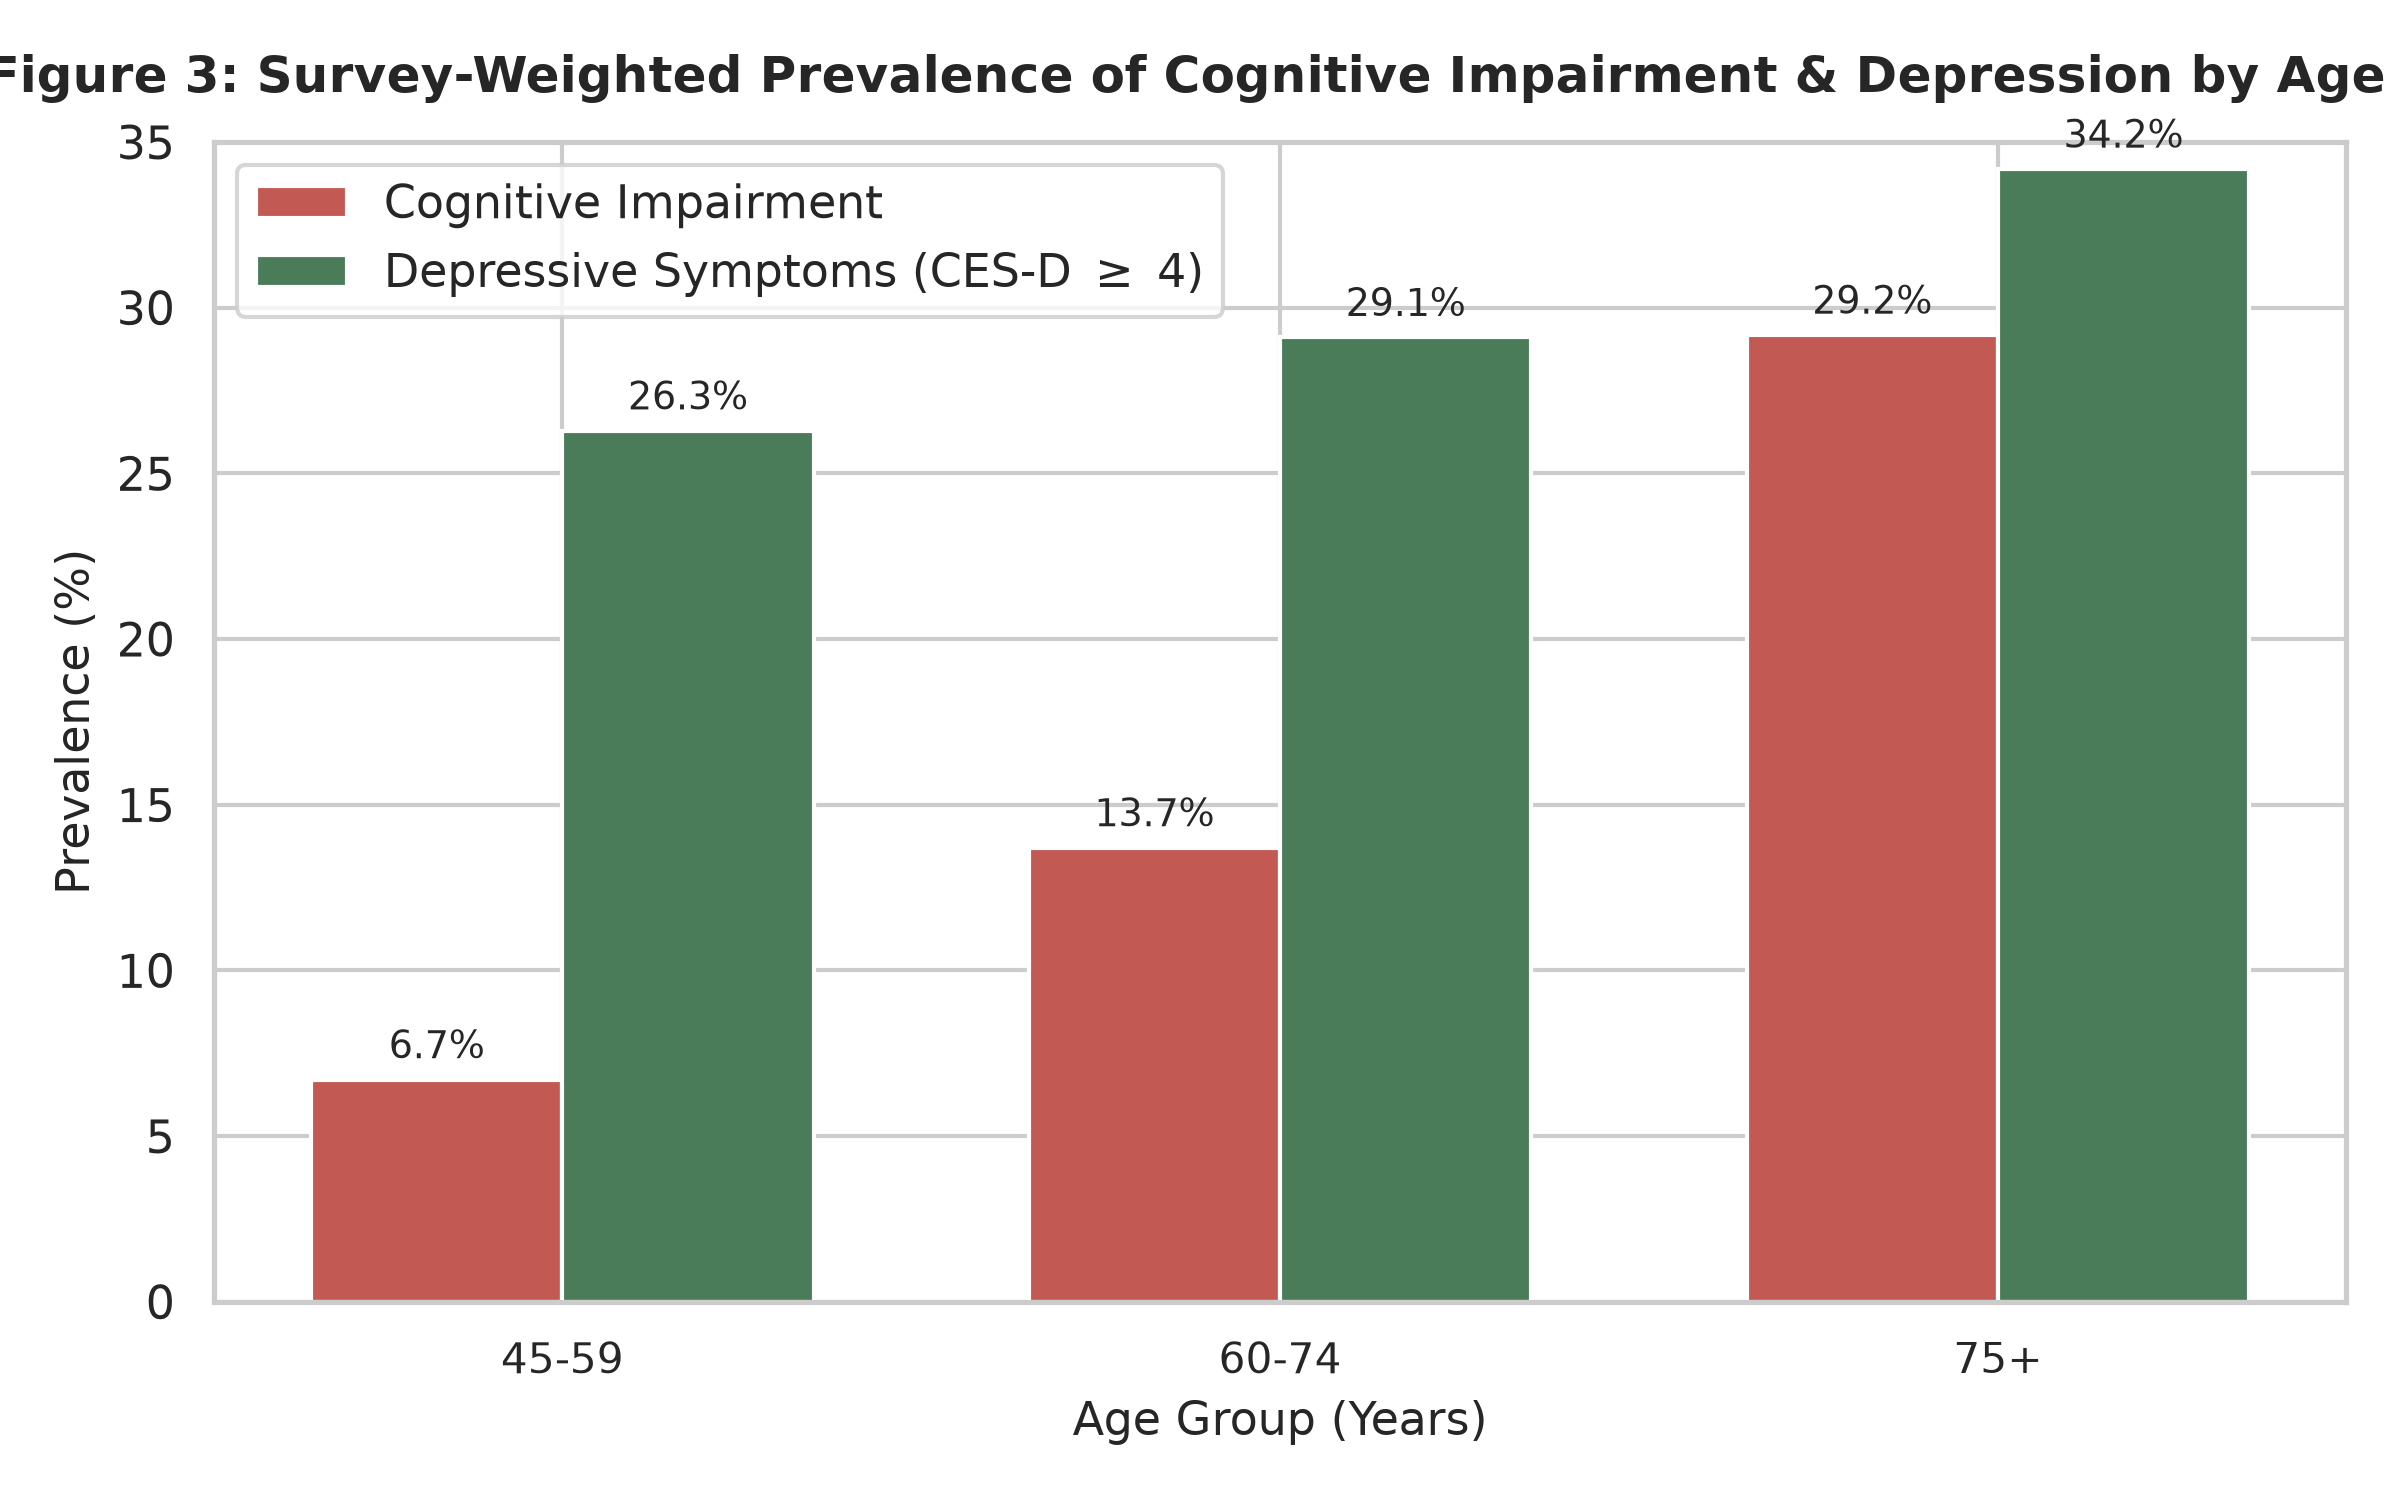
\includegraphics[width=0.72\textwidth]{figures/figure3_outcome_prevalence_by_age.png}
    \caption{\textbf{Prevalence of Cognitive Impairment and Depressive Symptoms across Age Strata.} Illustrates the sharp, non-linear acceleration of cognitive impairment compared to the steady rise in depressive symptoms.}
    \label{fig:outcomes_age}
\end{figure}

The patterns reveal key differences between cognitive and affective ageing:
\begin{enumerate}
    \item \textbf{Cognitive Impairment Accelerates Dramatically:} In mid-life (45--59), the prevalence of low memory-orientation performance is relatively low at 7.61\% (95\% CI: 7.00--8.22). It doubles to 15.61\% (95\% CI: 14.58--16.65) among the young-old (60--74), and quadruples to \textbf{28.85\%} (95\% CI: 26.20--31.50) among the oldest-old (75+). The continuous memory-orientation score similarly drops from a mean of $17.01$ points in mid-life to $13.88$ points among adults aged 75+.
    \item \textbf{Depression Shows a Chronic, Elevated Baseline:} Unlike cognition, depressive symptoms are highly prevalent even in mid-life, affecting 26.28\% of adults aged 45--59. The prevalence rises moderately to 29.10\% in young-old age and reaches \textbf{34.18\%} among the oldest-old. This indicates that late-life depression in India is not merely an acute consequence of advanced decrepitude; it represents an expansive, lifelong mental health burden.
\end{enumerate}

\begin{table}[!htbp]
\centering
\begin{singlespace}
\small
\caption{\textbf{Survey-Weighted Prevalence and Domain Means of Health Outcomes across Age Strata (Design-Based 95\% CIs).}}
\label{tab:outcomes_age}
\renewcommand{\arraystretch}{0.95}
\resizebox{0.95\textwidth}{!}{%
\begin{tabular}{llrrr}
\toprule
\textbf{Age Group} & \textbf{Outcome Measure} & \textbf{Weighted Estimate} & \textbf{95\% Confidence Interval} & \textbf{Sample N} \\
\midrule
45--59 years & Cognitive impairment (\%) & 7.61\% & (7.00\% -- 8.22\%) & 32,301 \\
45--59 years & Depressive symptoms (\%) & 26.28\% & (24.99\% -- 27.58\%) & 34,009 \\
45--59 years & Mem+orient score (mean, 0--28) & 17.01 & (16.85 -- 17.17) & 32,301 \\
45--59 years & CES-D score (mean, 0--10) & 2.86 & (2.81 -- 2.91) & 34,009 \\
\midrule
60--74 years & Cognitive impairment (\%) & 15.61\% & (14.58\% -- 16.65\%) & 22,223 \\
60--74 years & Depressive symptoms (\%) & 29.10\% & (27.80\% -- 30.41\%) & 24,370 \\
60--74 years & Mem+orient score (mean, 0--28) & 15.51 & (15.38 -- 15.65) & 22,223 \\
60--74 years & CES-D score (mean, 0--10) & 3.01 & (2.95 -- 3.06) & 24,370 \\
\midrule
75+ years & Cognitive impairment (\%) & 28.85\% & (26.20\% -- 31.50\%) & 5,257 \\
75+ years & Depressive symptoms (\%) & 34.18\% & (31.02\% -- 37.33\%) & 6,446 \\
75+ years & Mem+orient score (mean, 0--28) & 13.88 & (13.65 -- 14.11) & 5,257 \\
75+ years & CES-D score (mean, 0--10) & 3.27 & (3.15 -- 3.39) & 6,446 \\
\midrule
\textbf{Full Population} & \textbf{Cognitive impairment (\%)} & \textbf{12.79\%} & \textbf{(12.03\% -- 13.54\%)} & \textbf{59,781} \\
\textbf{Full Population} & \textbf{Depressive symptoms (\%)} & \textbf{28.24\%} & \textbf{(27.19\% -- 29.28\%)} & \textbf{64,825} \\
\textbf{Full Population} & \textbf{Mem+orient score (mean)} & \textbf{16.13} & \textbf{(16.00 -- 16.25)} & \textbf{59,781} \\
\textbf{Full Population} & \textbf{CES-D score (mean)} & \textbf{2.96} & \textbf{(2.92 -- 3.00)} & \textbf{64,825} \\
\bottomrule
\end{tabular}%
}
\end{singlespace}
\end{table}

\subsection{Demographic Variations: Gender, Urban-Rural, and Caste Disparities}
To understand how these outcomes vary across India's social landscape, Table~\ref{tab:demo_variation} reports the adjusted associations of key demographic characteristics with cognitive impairment and depressive symptoms from multivariable demographic models (Model A specification).

\begin{table}[!htbp]
\centering
\begin{singlespace}
\small
\caption{\textbf{Associations of Demographic Factors with Cognitive Impairment and Depressive Symptoms (Model A Specifications).}}
\label{tab:demo_variation}
\renewcommand{\arraystretch}{0.95}
\resizebox{\textwidth}{!}{%
\begin{tabular}{llcc}
\toprule
\textbf{Health Outcome} & \textbf{Demographic Factor (Contrast)} & \textbf{Prevalence Ratio (95\% CI)} & \textbf{\textit{p}-value} \\
\midrule
\textbf{Cognitive Impairment} & Female (vs. Male) & 1.93 (1.77 -- 2.09) & $<0.001$ \\
\textbf{Cognitive Impairment} & Urban Residence (vs. Rural) & 0.44 (0.38 -- 0.53) & $<0.001$ \\
\textbf{Cognitive Impairment} & Other Backward Classes (vs. General) & 1.24 (1.10 -- 1.39) & $<0.001$ \\
\textbf{Cognitive Impairment} & Scheduled Caste (vs. General) & 1.63 (1.45 -- 1.83) & $<0.001$ \\
\textbf{Cognitive Impairment} & Scheduled Tribe (vs. General) & 2.12 (1.85 -- 2.43) & $<0.001$ \\
\textbf{Cognitive Impairment} & Chronological Age (per year increase) & 1.05 (1.04 -- 1.05) & $<0.001$ \\
\midrule
\textbf{Depressive Symptoms} & Female (vs. Male) & 1.19 (1.12 -- 1.26) & $<0.001$ \\
\textbf{Depressive Symptoms} & Urban Residence (vs. Rural) & 0.94 (0.85 -- 1.04) & $0.203$ \\
\textbf{Depressive Symptoms} & Other Backward Classes (vs. General) & 1.14 (1.04 -- 1.24) & $0.003$ \\
\textbf{Depressive Symptoms} & Scheduled Caste (vs. General) & 1.26 (1.16 -- 1.36) & $<0.001$ \\
\textbf{Depressive Symptoms} & Scheduled Tribe (vs. General) & 1.01 (0.89 -- 1.15) & $0.866$ \\
\textbf{Depressive Symptoms} & Chronological Age (per year increase) & 1.01 (1.00 -- 1.01) & $<0.001$ \\
\bottomrule
\end{tabular}%
}
\end{singlespace}
\end{table}

The demographic patterns illuminate profound structural inequalities in health:
\begin{itemize}
    \item \textbf{The Massive Gender Penalty in Cognition:} Older Indian women have a \textbf{93\% higher prevalence} of low memory-orientation performance compared to older men ($\text{APR} = 1.93$, 95\% CI: 1.77--2.09, $p < 0.001$), after adjusting for age, caste, and state of residence. This striking disparity reflects historical patriarchal norms that prioritized boys' schooling and intellectual engagement while confining girls to domestic labor without literacy exposure. Women also experience 19\% higher depressive symptom rates ($\text{APR} = 1.19, p < 0.001$).
    \item \textbf{The Urban Protective Gradient in Cognition:} Older adults living in urban towns and cities have a \textbf{56\% lower prevalence} of cognitive impairment compared to their rural counterparts ($\text{APR} = 0.44$, 95\% CI: 0.38--0.53, $p < 0.001$). Urban environments historically provided better access to schools, libraries, public transport, and diverse social cognitive stimulation.
    \item \textbf{The Caste Gradient:} Scheduled Tribe (ST) adults face more than double the cognitive impairment rate of General caste peers ($\text{APR} = 2.12$, $p < 0.001$), while Scheduled Caste (SC) adults face a 63\% higher rate ($\text{APR} = 1.63$, $p < 0.001$). For depression, SC adults experience a 26\% elevated prevalence ($\text{APR} = 1.26, p < 0.001$).
\end{itemize}
